\documentclass[a4paper, 12pt]{article}
\usepackage[spanish]{babel}
\usepackage{graphicx}

\usepackage{amsmath, amsthm, amssymb}


\begin{document}
\title{Moogle!}
\author{Jossué Arteche Muñoz, C111}
\maketitle

\section{Introducción}
El proyecto “Moogle!” es una aplicación cuyo propósito es buscar inteligentemente un texto en un conjunto de documentos. Dicha aplicacion funciona con un motor que implementa un algoritmo de búsqueda, y otras funcionalidades como operadores de búsqueda, sugerencias de posibles entradas etc. En este informe se expondrá el funcionamiento general del programa y las instrucciones de cómo usarlo.

Un motor de búsqueda debe tener, para brindar al usuario la mejor experiencia posible, diversas características. Primero que todo, debe ser capaz de obtener la información que el usuario introduce en el buscador, luego, y quizás esto sea lo más esencial, debe ser capaz de retornar los documentos más útiles para el usuario, y como es lógico, en orden descendente de relevancia, de forma tal que el primer documento que vea el usuario sea el más relevante.

El problema más complicado de resolver es el segundo. Uno podría tener la idea de recorrer todos los libros buscando la entrada del usuario, pero eso sería extremadamente ineficiente, sería como leer todos los libros cada vez que se quiera buscar algo. Afortunadamente existen soluciones más prácticas.

\section{Funcionamiento General}
Moogle! utiliza un modelo de recuperación de información denominado “modelo vectorial”. La idea de la que parte este modelo es de expresar cada documento, y la pregunta o query como vectores n-dimensionales, donde n es la cantidad de palabras de nuestro directorio de documentos, y cada dimensión i está representada por el valor de relevancia de la i-ésima palabra.

Para calcular la relevancia se usa el valor tf-idf (term frecuency – inverse term frecuency) de cada palabra, el cual, a grandes rasgos es un valor directamente proporcional a la cantidad de veces que aparece una palabra e inversamente proporcional a la cantidad de documentos en los que aparece. De esta forma se garantiza que palabras muy comunes, que aparecen en muchos documentos tengan una relevancia baja.

Retomando el modelo vectorial, la idea de expresar a los documentos y a la query como vectores es muy útil ya que es posible calcular la similitud entre dos vectores mediante el valor del coseno del ángulo comprendido, ya que mientras mas cercano a 1 el valor del coseno mas cercano a 0 es el ángulo y mas similares son ambos vectores. De esta forma tenemos una manera de devolver los documentos mas relevantes según una búsqueda.

\section{Estructura de la Implementación}
Primero debemos expresar cada vector como documento. Para ello necesitamos el valor tf-idf de cada palabra en cada documento. Para esto necesitamos saber cuántas veces se repite cada palabra en cada documento y en cuántos documentos se repite, y además obtenerlo de la forma más eficiente posible. Necesitamos información que es particular del directorio. Para esto se implementó una clase llamada “TfIdfDirectory” la cuál contendrá todo lo relacionado a nuestro directorio objetivo. Cuando se construye un objeto TfIdfDirectory se crea una estructura que relaciona cada palabra y los documentos en los que aparece, y a su vez relaciona estos con las posiciones en las que aparece cada palabra en dicho documento. Con este objetivo se usa un diccionario de diccionarios. Este objeto será muy útil, pues a partir de la informacion que poporciona, calcular el tf-idf de una palabra se reduce a preguntar la cantidad de llaves de un diccionario, estructura que además reduce el orden del algoritmo considerablemente. Esta estructura se construye linealmente con el metodo de una clase estática, WordsIndexer.GetWordsIndexes recorriendo todos los documentos una y solo una vez. Una vez se tienen las palabras indexadas ya se puede crear cada vector documento, calculando el tf-idf de cada palabra con funciones que estan implementadas dentro de la clase TfIdfDirectory, de forma muy sencilla. Una vez obtenidas las palabras indexadas y el conjunto de vectores de la base de datos, queda construido el objeto TfIdfDirectory de nuestro direcotrio objetivo y ya se pueden realizar todas las búsquedas deseadas
\begin{figure}
    \center
    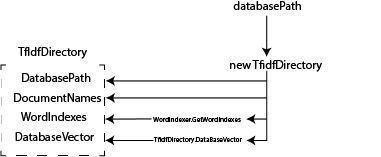
\includegraphics[width=10cm]{RepresentacionDelPrecalculo.png}
\end{figure}

Cuando se introduce una búsqueda, esta se convierte en un vector n-dimensional, y se calcula su similitud coseno con todos los vectores documento. Luego se seleccionan los 5 documentos de mayor similitud y se devuelven como resultado. De esta forma se obtienen búsquedas de forma rápida y eficiente.

\begin{figure}
    \center
    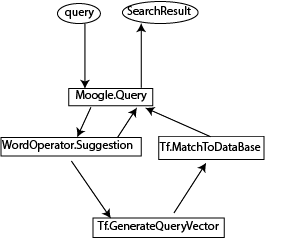
\includegraphics[width=6cm]{DiagramaDeClases.png}
\end{figure}

Es importante aclarar que lo que se guarda como llave en el diccionario no es la palabra en si, si no su forma simple. Como forma simple se considerará a la palabra en minúsculas y sin tilde. Por ejemplo, las palabras “Ordenación” y “ordenación” se guardan bajo la misma llave, “ordenacion”. Para esto se ha implementado la clase estatica WordOperator, que contiene métodos como ConvertToSimpleVersion () y otros útiles relacionados con palabras que tambien utiliza la implementación de Moogle!.

\section{Otras Funcionalidades}
Moogle! también cuenta con otras funcionalidades interesantes como los operadores de busqueda:
\begin{itemize}
    \item Se puede poner ``!'' antes de una palabra para que no aparezca en los documentos devueltos.
    \item Poner ``\^{}''  antes de una palabra hará que obligatoriamente aparezca en los documentos devueltos.
    \item Poner ``*'' varias veces antes de una palabra aumentara su relevancia en la query.
    \item Poner ``\~{}'' entre dos palabras hará que obligatoriamente aparecan los documentos que contienen ambas palabras cerca
\end{itemize}
Para la implementacion de estos operadores, básicamente se asocia cada dimensión del vector query con su operacion correspondiente (que puede ser vacia), y en dependencia de esta se alteran los valores de la similitud coseno para forzar al algoritmo a devolver los valores esperados. (Por ejemplo, si la palabra de la dimension i tiene la operacion ! y la i-esima dimension del j-ésimo vector es distinta de cero, como la palabra no debe aparecer en ese documento entonces la similitud entre ambos sera 0)

Moogle! también es capaz de dar una vista previa del documento, un snippet, que aparecera debajo del nombre del resultado. Como ya se guardo en un diccionario las posiciones en donde aparecía una palabra en un documento, esta funcionalidad es sencilla de implementar. Para ello se toma la
palabra mas relevante de la query y se busca la mediana de las posiciones en las que se eencuentra de aparecer en el documento y se toma un fragmento que tiene a dicha palabra en el centro.

El programa tambien es capaz de dar sugerencias. En caso de que se introduzca una palabra que no se encuentre en el directorio entonces se busca la palabra mas similar de entre todas las palabras que si contiene (dicha similitud se calcula usando distancia de levenshtein), luego se sustituye esa posible palabra en la query y se vuelve a realizar la busqueda, obteniendo los resultados sugeridos.

\section{Clases Implementadas}
\begin{itemize}
	\item Moogle: Esta clase estática realiza las búsquedas.
	\item WordsIndexer: Clase estática que crea el diccionario de las palabras de la base de documentos.
	\item WordOperator: contiene funciones relacionadas con el tratamiento de las palabras, como reducirlas a su forma simple, entre otras.
	\item TfIdfDirectory: esta clase contiene como propiedades al diccionario de la base de documentos, así como la matriz de los vectores documento. También contiene funciones para el cálculo del tf-idf, la similitud coseno, el snippet, etc.
	\item QueryDimension: los objetos de este tipo guardan la palabra asociada a la dimensión del vector query, así como su respectivo valor tf-idf y la operación que se realiza sobre él.
	\item SimilarityResult: un objeto de este tipo guardara la similitud coseno de la query con un documento, y el índice de este documento.
	\item WordOperation: clase abstracta de la que heredan las dsitintas clases de operaciones de búsqueda:
	\begin{itemize}
	\item OpNone: clase que representa la ausencia de operaciones
	\item OpMustNotbe: clase que representa la operación ``!''
	\item OpMustBe: clase que representa la operación ``\^{}''
	\item OpIsRelevant: clase que representa la operación ``*''
	\item OpIsCloseTo: clase que representa la operación ``\~{}'' 
	\end{itemize}
\end{itemize}

\section{Conclusiones}
Podemos concluir que la implementación del modelo vectorial, como modelo de recuperación de la información. Estos arrojan resultados satisfactorios (búsquedas en un quinto de segundo como promedio) para una cantidad aproximada de 50 MB de texto plano, distribuidos en 35 libros, con una capacidad de computo mínima. También se puede constatar la utilidad de los diccionarios para almacenar objetos, ya que no afectan al orden del algoritmo y garantizan su eficiencia.
\end{document}